\section{DVI encoder}

\marginpar{Include formula for exact throughput, and pixel clocks used for OV7670}

The \gls{dvi} encoder and decoder presented here are based heavily upon a reference design provided by Digilent's IP library for the Zybo development board. Rather than reinvent the wheel, this project opts to use these cores as a base and extend them for use with image sensors. All third-party code has been attributed, as per the BSD-license which the IP is released under. Custom additions have been marked.

\subsection{\texttt{rgb2dvi} module overview}
\begin{figure}
  \centering
  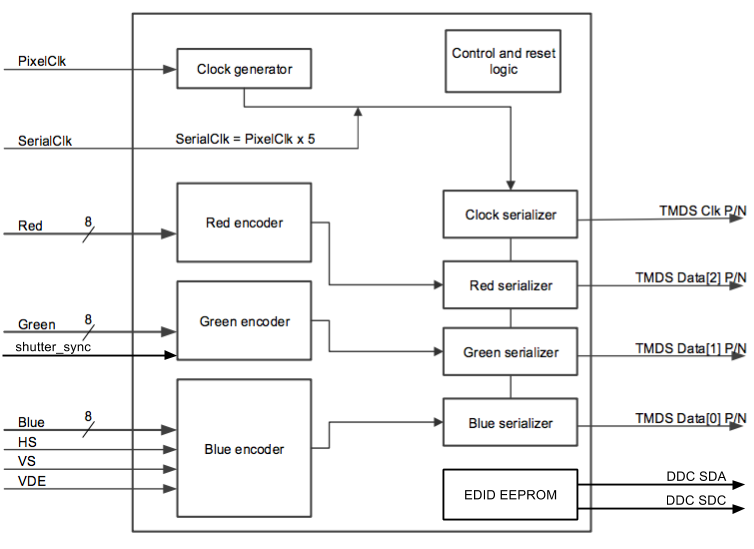
\includegraphics[width=1\textwidth]{./img/rgb2dvi.png}\par
  Source: \url{https://github.com/DigilentInc/vivado-library/blob/master/ip/rgb2dvi_v1_2/docs/rgb2dvi_v1_2.pdf}
  \caption{Block diagram of the DVI encoder.}
  \label{fig:rgb2dvi}
\end{figure}

The \gls{dvi} encoder takes a 24-bit wide pixel data bus as the main input, splitting off into three 8-bit channels for Red, Green and Blue. As the application requires a RAW pixel format instead of RGB we must deviate from the \gls{dvi} specification slightly by combining all channels into one large input, however internally they are still treated separately. Only a single channel (Blue) is used for data in the proof-of-concept as the OV7670 only has an 8-bit \gls{adc}, however the Green channel is also used to transmit the control signals related to flash and shutter synchronisation. Combining all channels gives a maximum pixel depth of 24-bits --- the image sensor on a professional \gls{dslr} will typical have a 12--14-bit \gls{adc}, so 24-bits is more than sufficient. Alongside the pixel bus are the regular video timing and synchronisation signals used elsewhere in the design. In addition to these timing signals, a \texttt{shutter\_sync} signal has been added which fires just before each new frame so that the receiver side can sequence a mechanical shutter or flash if present. Much like the video timing signals, the shutter synchronisation signal is sent via the control bits on the Green channel.

Internally the \gls{dvi} encoder instantiates three identical \texttt{TMDS\_encoder} blocks and assigns each one to a channel. Immediately after each \gls{tmds} encoder is an \texttt{OutputSERDES} block which is what actually drives the \gls{tmds}-encoded data across the interface. Listing \ref{lst:encoder_instances} shows how the \texttt{generate} statement is used to create three identical instances of the \texttt{TMDS\_encoder} and \texttt{OutputSERDES} blocks.

\begin{lstlisting}[caption={Instantiatiating a TMDS encoder and serialiser for each channel.}, label={lst:encoder_instances}, language=VHDL]
DataEncoders: for i in 0 to 2 generate
   DataEncoder: entity work.TMDS_Encoder
      port map (
         PixelClk => PixelClk,
         SerialClk => SerialClk,
         pDataOutRaw => pDataOutRaw(i),
         aRst => pRstLck,
         pDataOut => pDataOut(i),
         pC0 => pC0(i),
         pC1 => pC1(i),
         pVde => pVde(i)
      );
   DataSerializer: entity work.OutputSERDES
      generic map (
         kParallelWidth => 10) -- TMDS uses 1:10 serialization
      port map(
         PixelClk => PixelClkIO,
         SerialClk => SerialClkIO,
         sDataOut_p => TMDS_Data_p(i),
         sDataOut_n => TMDS_Data_n(i),
         --Encoded parallel data (raw)
         pDataOut => pDataOutRaw(i),
         aRst => pRstLck);      
end generate DataEncoders;
\end{lstlisting} 

\subsection{TMDS encoding}
As covered in the section on the \gls{dvi} interface, \gls{tmds} encoding is utilised in order to minimise data transitions (and thus \gls{emi}) and provide a \gls{dc} balance, which it does by mapping each 8-bit input to a unique 10-bit \gls{tmds} character.

The flowchart in Figure \ref{fig:tmds_encoding_algorithm} outlines the algorithm used for \gls{tmds} encoding. The notation is as follows (\url{https://web.archive.org/web/20120521030851/http://www.ddwg.org/lib/dvi_10.pdf}):
\begin{itemize}
    \item \texttt{D C0 C1 DE}: The input set of the encoder. D is an 8-bit pixel data value, C0 and C1 are the two control bits and DE indicates whether the data is valid.
    \item \texttt{cnt}: This register indicates the disparity of the data stream. A value \texttt{1} in the bit stream will increment the counter, and a \texttt{0} will decrement it. \texttt{cnt(t-1)} refers to the register value for the previous bit of data, and \texttt{cnt(t)} is the register value for the current bit of input data.
    \item \texttt{q\_out}: The \gls{tmds}-encoded output value.
    \item N\textsubscript{1}\{x\}: Number of \texttt{1}s in \texttt{x}.
    \item N\textsubscript{0}\{x\}: Number of \texttt{0}s in \texttt{x}.
\end{itemize}

The encoding algorithm can be split into three discrete pipeline stages:
\begin{enumerate}
    \item Transition minimisation
    \item DC balancing
    \item Output registering
\end{enumerate}

\begin{lstlisting}[caption={TMDS encoder transition minimisation stage.}, label={lst:encoder_stage_1}, language=VHDL]
-- Pipeline stage 1, minimise transitions
----------------------------------------------------------------------------------
Stage1: process(PixelClk)
begin
    if Rising_Edge(PixelClk) then
        pVde_1 <= pVde;

        n1d_1 <= sum_bits(pDataOut(7 downto 0));
        pDataOut_1 <= pDataOut; --insert data into the pipeline;
        pC0_1 <= pC0; --insert control into the pipeline;
        pC1_1 <= pC1;
    end if;
end process Stage1;

----------------------------------------------------------------------------------
-- Choose one of the two encoding options based on n1d_1
----------------------------------------------------------------------------------
q_m_xor_1(0) <= pDataOut_1(0);
encode1: for i in 1 to 7 generate
    q_m_xor_1(i) <= q_m_xor_1(i-1) xor pDataOut_1(i);
end generate encode1;
q_m_xor_1(8) <= '1';

q_m_xnor_1(0) <= pDataOut_1(0);
encode2: for i in 1 to 7 generate
    q_m_xnor_1(i) <= q_m_xnor_1(i-1) xnor pDataOut_1(i);
end generate encode2;
q_m_xnor_1(8) <= '0';

q_m_1 <= q_m_xnor_1 when n1d_1 > 4 or (n1d_1 = 4 and pDataOut_1(0) = '0') else
         q_m_xor_1;

n1q_m_1 <= sum_bits(q_m_1(7 downto 0));
\end{lstlisting}

The first stage, in Listing \ref{lst:encoder_stage_1} aims to minimise the number of transitions in the data by XORing with previous inputs. After counting the ones and zeros in the input bits, the intermediate \texttt{q\_m} bits are set by XORing them with the current data bits. An additional 9\textsuperscript{th} intermediate bit is set to either \texttt{1} if the input data contains less than four ones, or \texttt{0} otherwise.

\begin{lstlisting}[caption={TMDS encoder DC balancing stage.}, label={lst:encoder_stage_2}, language=VHDL]
----------------------------------------------------------------------------------
-- Pipeline stage 2, balance DC
----------------------------------------------------------------------------------
Stage2: process(PixelClk)
begin
    if Rising_Edge(PixelClk) then
        n1q_m_2 <= n1q_m_1;
        n0q_m_2 <= 8 - n1q_m_1;
        q_m_2 <= q_m_1;
        pC0_2 <= pC0_1;
        pC1_2 <= pC1_1;
        pVde_2 <= pVde_1;
    end if;
end process Stage2;

cond_balanced_2 <=   '1' when cnt_t_3 = 0 or n1q_m_2 = 4 else -- DC balanced output
                           '0';
cond_not_balanced_2 <=  '1' when (cnt_t_3 > 0 and n1q_m_2 > 4) or -- too many 1's
                                     (cnt_t_3 < 0 and n1q_m_2 < 4) else -- too many 0's
                        '0';

control_token_2 <=  kCtlTkn0 when pC1_2 = '0' and pC0_2 = '0' else
                     kCtlTkn1 when pC1_2 = '0' and pC0_2 = '1' else
                     kCtlTkn2 when pC1_2 = '1' and pC0_2 = '0' else
                     kCtlTkn3;
                            
q_out_2 <=  control_token_2                                             when pVde_2 = '0' else  --control period
               not q_m_2(8) & q_m_2(8) & not q_m_2(7 downto 0)    when cond_balanced_2 = '1' and q_m_2(8) = '0' else
               not q_m_2(8) & q_m_2(8) & q_m_2(7 downto 0)        when cond_balanced_2 = '1' and q_m_2(8) = '1' else
               '1' & q_m_2(8) & not q_m_2(7 downto 0)             when cond_not_balanced_2 = '1' else
               '0' & q_m_2(8) & q_m_2(7 downto 0);  --DC balanced

dc_bias_2 <= signed('0' & n0q_m_2) - signed('0' & n1q_m_2);

cnt_t_2 <=  to_signed(0, cnt_t_2'length)                                   when pVde_2 = '0' else   --control period
               cnt_t_3 + dc_bias_2                                            when cond_balanced_2 = '1' and q_m_2(8) = '0' else
               cnt_t_3 - dc_bias_2                                            when cond_balanced_2 = '1' and q_m_2(8) = '1' else
               cnt_t_3 + signed('0' & q_m_2(8 downto 8) & '0') + dc_bias_2     when cond_not_balanced_2 = '1' else
               cnt_t_3 - signed('0' & not q_m_2(8 downto 8) & '0') - dc_bias_2;
\end{lstlisting}

A second stage, shown in Listing \ref{lst:encoder_stage_2}, aims to balance the overall \gls{dc} offset of the bit stream. If the \texttt{VDE} signal is low then this step is bypassed altogether as this indicates that we are now in the blanking period and should only be sending control data. During the blanking period the input pixel data is completely ignored, instead the control signals are encoded directly using a \gls{lut} to produce one of four unique 10-bit control tokens, depending on the relevant combination of control inputs \texttt{C0} and \texttt{C1}. These control tokens have been specially picked to be easy to detect at the receiver in order to aid phase alignment. If we are in the active video period then the process is significantly more complex and involves counting the number of ones and zeros in the intermediate values to determine what value to clock into the output registers.

The stage of the pipeline clocks the intermediate values into an output register, \texttt{q\_out}, where they are then passed on to the serialiser.

\subsection{Serialisation}

Originally written in VHDL, the serialiser code was re-written in Verilog as part of this project. To obtain the highest data rates that the \gls{fpga} is capable of it is necessary to use Xilinx's OSERDESE2 primitives, which take the 10-bit output characters from the \gls{tmds} encoder and two clocks (one parallel clock and a serial higher serial clock) and then serialises them into a single-bit high-speed output stream. The OSERDESE2 primitive only has an 8-bit input which is too narrow for the 10-bit \gls{tmds} output. To achieve the 10:1 serialisation ratio required, two OSERDESE2 primitives operating in \gls{ddr} mode must be chained together as in Figure \ref{fig:10_1_serdes}. The inputs to the OSERDESE2 primitives are swapped as \gls{dvi} sends the least significant bit first, whereas the OSERDESE2 primitives send \texttt{D1} first.

When configured as a cascaded 10:1 \gls{ddr} topology the OSERDESE2 primitive has an output latency of 5 clock cycles (\url{http://www.xilinx.com/support/documentation/user_guides/ug471_7Series_SelectIO.pdf}). To ensure that the \gls{tmds} clock channel is correctly aligned with the data channels it is also run through a serialiser, adding 5 cycles of latency to bring it back in line with the rest of the data.

\begin{figure}
  \centering
  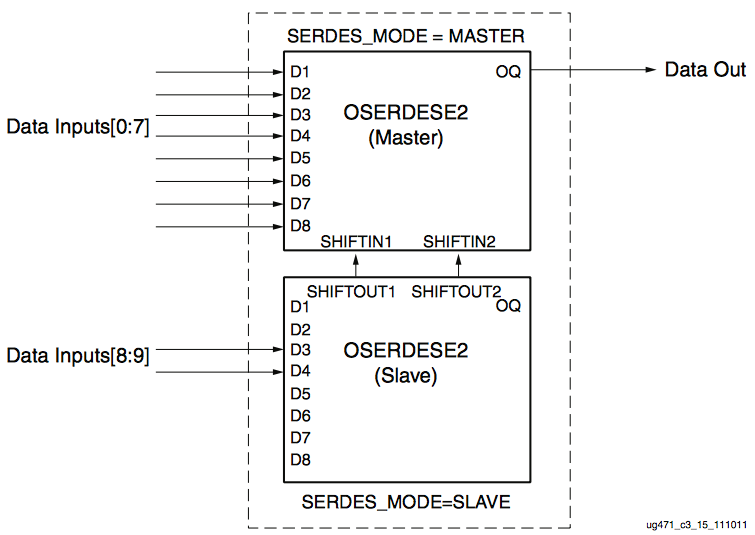
\includegraphics[width=1\textwidth]{./img/10_1_serdes.png}\par
Source: \url{http://www.xilinx.com/support/documentation/user_guides/ug471_7Series_SelectIO.pdf}
  \caption{10:1 serialisation is achieved by chaining two OSERDES2 primitives in DDR mode.}
  \label{fig:10_1_serdes}
\end{figure}

\subsection{DDC channel}

While the video sink is usually the I\textsuperscript{2}C master of the \gls{ddc} channel, the proof-of-concept design instead assigns the video source (image sensor) as the master so that it may advertise its capabilities to the camera body. The \gls{ddc} code is part of Digilent's IP library and uses internal memory resources to store a 128-byte \gls{edid} and presents itself as an I\textsuperscript{2}C-attached \gls{eeprom}. The \gls{edid} implementation is detailed in Section \ref{sec:edid}.

\subsection{Clocking}
Three clocks --- all of which are generated externally --- are required for the \gls{dvi} encoder to function correctly:
\begin{itemize}
    \item \texttt{PixelClk}: One tick for every pixel
    \item \texttt{SerialClk}: Feeds the OSERDESE2 primitives, must be 5x the frequency of the PixelClk due to the 10:1 serialisation ratio and use of \gls{ddr} mode
    \item \texttt{RefClk}: Drives the I\textsuperscript{2}C-attached \gls{eeprom} for the \gls{edid}
\end{itemize}

The route between the serial clock and the OSERDESE2 primitives is without doubt the most critical part of the entire design as it limits the maximum throughput. To ensure that the tools have the best possible chance of meeting the throughput requirements the serial clock is constrained to be five times the pixel clock frequency, as in Listing \ref{lst:timing_constraints}

\begin{lstlisting}[caption={Serial clock timing constraints}, label={lst:timing_constraints}, language=tcl]
### Clock constraints ###
create_generated_clock -source [get_ports PixelClk] -multiply_by 5 [get_ports SerialClk]
\end{lstlisting}

\subsection{Performance}
Performance is ultimately limited by the Zynq-700's F\textsubscript{MAX\_BUFIO} figure, specified as \SI{710}{\mega\hertz}\cite{xilinx:ds187}. F\textsubscript{MAX\_BUFIO} is the maximum switching rate of the input / output clock tree, meaning that any IO buffers cannot operate any higher than \SI{710}{\mega\hertz}. The highest resolution is thus the one which corresponds to a pixel clock of \SI{142}{\mega\hertz}, which is just shy of the \SI{148.5}{\mega\hertz} pixel clock required for 1080p. Because silicon vendors are normally conservative with their specifications, it turns out that even though the timing constraints are not met during place and route, the Zybo development board used for the proof-of-concept can actually operate outside of its specification, and can just about manage to transmit and receive 1080p video.